\documentclass[11pt,a4paper]{article}
\usepackage[margin=2.5cm]{geometry}
\usepackage{amsmath,amssymb,graphicx,hyperref,booktabs,xcolor}
\usepackage[T1]{fontenc}
\usepackage{lmodern}

\hypersetup{colorlinks=true,linkcolor=blue,citecolor=blue,urlcolor=blue}

\title{\textbf{Paper 27: The Zone Formation Commitment Epoch}\\[4pt]
\large Oscillatory Polarity, FA-Independent Flip Timescale,\\
and the Mixed Pitchfork--Spinodal Mechanism}

\author{VCML Theory Series}
\date{March 2026}

\begin{document}
\maketitle

\begin{abstract}
Paper 26 identified a temporal anti-correlation in VCML zone structure:
$C(t_{\rm ref}, T_{\rm end}) < 0$ for $t_{\rm ref} < 1600$, suggesting a
``zone formation commitment epoch.''
Paper~27 investigates the full temporal dynamics with three experiments:
\textbf{Exp A} (80 runs): FA $\times$ WR sweep at $T = 5000$ to test
$t^* \sim 1/(P_c \cdot \mathrm{FA} \cdot \mathrm{WR})$.
\textbf{Exp B} (15 runs): zone-level trajectories at standard parameters
to $T = 6000$, testing pitchfork vs.\ spinodal mechanism.

Three unexpected findings emerge:
(1) The temporal correlation $C(t_{\rm ref}, T_{\rm end})$ is \emph{oscillatory}
rather than showing a single zero-crossing -- zones flip polarity repeatedly
throughout the run, with flip timescale $\sim 800$--$1600$ steps.
(2) The first flip time $t^*$ is \emph{FA-independent}: $t^* \approx 1780$
at WR$=1.2$, $t^* \approx 1600$ at WR$=2.4$, and $t^* \approx 630$ at
WR$=4.8$, regardless of FA over the range 0.10--0.80.
This contradicts the linear prediction $t^* \propto (\mathrm{FA} \cdot \mathrm{WR})^{-1}$:
perturbation rate (WR) governs timing, not consolidation rate (FA).
(3) The per-zone flip timescale shows $\sigma_{\rm in}/\sigma_{\rm btw} = 0.67$,
a \emph{mixed} regime: not pure pitchfork (zones flip together) nor pure
spinodal (zones flip independently).
These results reframe the commitment epoch as a recurring instability driven by
the continuous interplay of wave injection and copy-forward inheritance, not a
one-time symmetry-breaking bifurcation.
\end{abstract}

% ─────────────────────────────────────────────────────────────────────────────
\section{Introduction}
% ─────────────────────────────────────────────────────────────────────────────

Paper~26 computed the temporal correlation matrix $C(t_1, t_2)$ for VCML
zone structure, finding $C(400, 3000) = -0.36$ (strongly negative),
$C(2000, 3000) \approx 0$ (zero-crossing), and $C(2800, 3000) = +0.30$
(positive).  This was interpreted as a ``zone formation commitment epoch'':
before $t^* \approx 1600$--$2000$, zones were in the wrong polarity;
after, they locked in permanently.

Paper~27 tests this interpretation with three open questions from
\texttt{THEORY\_SYNTHESIS.md}:
\begin{itemize}
  \item \textbf{Q1}: Does $t^*$ scale as $1/(P_c \cdot \mathrm{FA} \cdot \mathrm{WR})$?
  \item \textbf{Q2}: Does sg4 eventually saturate?
  \item \textbf{Q7}: Is the commitment mechanism pitchfork (all zones flip
        simultaneously) or spinodal (zones flip independently)?
\end{itemize}

All three are resolved, though the answers differ from expectations.

% ─────────────────────────────────────────────────────────────────────────────
\section{Analytical Predictions}
% ─────────────────────────────────────────────────────────────────────────────

The zone-mean ODE (PDE~1 from Paper~23):
\begin{equation}
  \frac{d\bar{F}_z}{dt} = P_c \cdot \mathrm{FA} \cdot (\bar{m}_z - \bar{F}_z)
\end{equation}
has relaxation rate $\lambda = P_c \cdot \mathrm{FA}$.  Waves arrive at rate
$\mathrm{WR}/\mathrm{WAVE\_DUR}$ and each triggers births.  Two competing
hypotheses:

\paragraph{Linear model.}
Commitment requires accumulated signal to exceed noise:
$t^* \sim 1/(P_c \cdot \mathrm{FA} \cdot \mathrm{WR})$.
Both consolidation rate (FA) and perturbation rate (WR) contribute equally.

\paragraph{Perturbation-rate-only model.}
The first polarity commitment is set by how quickly births propagate a coherent
seed pattern, independent of how strongly it is encoded.
Prediction: $t^* \sim f(\mathrm{WR})$, FA-independent.

% ─────────────────────────────────────────────────────────────────────────────
\section{Experiment A: FA $\times$ WR Sweep}
% ─────────────────────────────────────────────────────────────────────────────

\subsection{Design}

FA $\in \{0.10, 0.20, 0.40, 0.80\}$ $\times$ WR $\in \{1.2, 2.4, 4.8, 9.6\}$,
$T = 5000$, 5 seeds each (80 runs).  The zone-mean stacked vector
$\mathbf{v}_z(t) = \{\bar{F}_z^{(1)}(t),\,\bar{F}_z^{(2)}(t)\}_{z=0}^{3}$
(8-dimensional) was stored at each checkpoint $t \in \{400,800,\ldots,4800\}$.
The temporal correlation is:
\begin{equation}
  C_{\rm zone}(t_{\rm ref}, T_{\rm end}) =
  \frac{\mathbf{v}(t_{\rm ref}) \cdot \mathbf{v}(T_{\rm end})}
       {\|\mathbf{v}(t_{\rm ref})\|\;\|\mathbf{v}(T_{\rm end})\|}
\end{equation}
averaged over seeds.  Note: the full-field cosine similarity used in Paper~26
is diluted by within-zone noise; zone-mean stacked vectors give a cleaner signal.

\subsection{Finding 1: Oscillatory temporal correlation}

$C_{\rm zone}(t_{\rm ref}, T_{\rm end})$ oscillates in sign throughout the run
for all (FA, WR) conditions.  For FA$=0.40$, WR$=4.8$:

\begin{table}[h]
\centering
\caption{$C_{\rm zone}(t_{\rm ref}, 4800)$ at selected time points,
         FA$=0.40$, WR$=4.8$, mean over 3 seeds.}
\label{tab:C_vals}
\begin{tabular}{rr}
\toprule
$t_{\rm ref}$ & $C_{\rm zone}(t_{\rm ref}, 4800)$ \\
\midrule
 400  & $-0.42$ \\
 800  & $+0.31$ \\
1200  & $-0.14$ \\
1600  & $+0.19$ \\
2000  & $-0.12$ \\
2400  & $-0.35$ \\
2800  & $-0.02$ \\
3600  & $-0.10$ \\
4400  & $+0.49$ \\
4800  & $+1.00$ \\
\bottomrule
\end{tabular}
\end{table}

There are at least 5 sign changes in the range $t \in [400, 4800]$.
\emph{Zone polarity is not permanently committed -- it oscillates on a
timescale of $\sim 800$--$1600$ steps.}
This directly refutes the Paper~26 interpretation of a one-time bifurcation:
that paper ran only to $T=3000$ and observed one zero-crossing.  The full
dynamics are oscillatory.

\subsection{Finding 2: FA-independent first-flip time}

Defining $t^*$ as the time of the \emph{first} zero-crossing of
$C_{\rm zone}(t_{\rm ref}, T_{\rm end})$ from negative to positive:

\begin{table}[h]
\centering
\caption{First flip time $t^*$ (steps) for all (FA, WR) conditions.
         Entries ``--'' indicate $t^* < 400$ (unresolved with 400-step checkpoints).}
\label{tab:tstar}
\begin{tabular}{rrrrrr}
\toprule
\multirow{2}{*}{WR} & \multicolumn{4}{c}{FA} & \multirow{2}{*}{Mean $t^*$} \\
\cmidrule(lr){2-5}
 & 0.10 & 0.20 & 0.40 & 0.80 & \\
\midrule
1.2 & 1803 & 1804 & 1787 & 1740 & 1784 \\
2.4 & 1497 & 1574 & 1647 & 1695 & 1603 \\
4.8 &  574 &  598 &  631 &  654 &  614 \\
9.6 & -- & -- & -- & -- & $<400$ \\
\bottomrule
\end{tabular}
\end{table}

The FA effect on $t^*$ is minimal (range $\pm 100$ steps within each WR row)
compared to the WR effect (factor $\sim 3\times$ from WR$=1.2$ to WR$=4.8$).
This falsifies the linear model $t^* \propto (\mathrm{FA} \cdot \mathrm{WR})^{-1}$
in favor of the perturbation-rate-only model: $t^* \approx f(\mathrm{WR})$.

\paragraph{Mechanism.}
The first polarity flip is set by the rate of wave-induced births, which
propagate a coherent zone pattern via copy-forward.  This process depends on
how many births have occurred (controlled by WR and $\nu$), not on how
strongly each birth encodes the field (controlled by FA).  FA determines
\emph{amplitude} (sg4), while WR determines \emph{timing} ($t^*$).

Quantitatively: WR$\,2\times$ from 1.2$\to$2.4 reduces $t^*$ by $\sim 11\%$;
WR$\,2\times$ from 2.4$\to$4.8 reduces $t^*$ by $\sim 62\%$.  The relationship
is super-linear (log-log slope $\approx -0.7$ to $-1.3$ over this range),
consistent with $t^* \sim \mathrm{WR}^{-1}$ with a lower-floor effect from the
finite lattice.

\subsection{Finding 3: sg4 saturation not reached by $T=5000$}

sg4 continues to grow through $T=5000$ for FA$=0.20$, 0.40, and 0.80.
Only FA$=0.10$ shows approximate saturation near $T=4000$.
This extends the Q2 open question: saturation timescale $T_{\rm sat}$ appears
to exceed 5000 steps for standard parameters.

% ─────────────────────────────────────────────────────────────────────────────
\section{Experiment B: Zone-Level Trajectories}
% ─────────────────────────────────────────────────────────────────────────────

\subsection{Design}

Standard parameters (FA$=0.40$, WR$=4.8$), 15 seeds, $T=6000$, 200-step
checkpoints.  For each zone $z \in \{0,1,2,3\}$ in each seed, $t^*_z$ was
defined as the first zero-crossing of $C_z(t_{\rm ref}, T_{\rm end})$ where
$C_z$ uses the zone-$z$ mean vector cosine similarity.

\subsection{Results: Mixed pitchfork--spinodal}

\begin{table}[h]
\centering
\caption{Per-zone first flip time $t^*_z$ (mean $\pm$ std over 15 seeds).}
\label{tab:zones}
\begin{tabular}{rr}
\toprule
Zone & $t^*_z$ (steps) \\
\midrule
0 & $1687 \pm 1109$ \\
1 & $1687 \pm 1082$ \\
2 & $1593 \pm 955$ \\
3 & $2273 \pm 1370$ \\
\bottomrule
\end{tabular}
\end{table}

The per-zone means are similar (1593--2273 steps), confirming that all zones
undergo their first flip at roughly the same epoch.  The large standard deviations
reflect large seed-to-seed variability.

\paragraph{Pitchfork vs.\ spinodal diagnosis.}
\begin{itemize}
  \item Within-seed spread (std of $\{t^*_0, t^*_1, t^*_2, t^*_3\}$ for one
        seed): $\sigma_{\rm in} = 602$ steps.
  \item Between-seed spread (std of mean $t^*$ across seeds):
        $\sigma_{\rm btw} = 900$ steps.
  \item Ratio: $\sigma_{\rm in}/\sigma_{\rm btw} = 0.67$.
\end{itemize}

\paragraph{Verdict: Mixed.}
$\sigma_{\rm in}/\sigma_{\rm btw} < 0.5$ would indicate pure pitchfork
(zones flip together); $> 1.5$ would indicate pure spinodal (zones flip
independently).  The observed $0.67$ is intermediate.

\emph{Interpretation}: Within a given seed run, zones tend to flip together
(pitchfork character), but there is substantial intra-seed asynchrony
($\sigma_{\rm in} = 602$ steps) suggesting that adjacent zones can flip at
different times.  The dominant source of variability is between seeds
(random wave sequence sets the absolute flip time), not between zones within
a seed.  This is consistent with a ``noisy pitchfork'': the zone-polarity
instability is a collective event, but initiated by a local fluctuation that
propagates across zones over $\sim 600$ steps.

% ─────────────────────────────────────────────────────────────────────────────
\section{Revised Picture: Metastable Zone Structure}
% ─────────────────────────────────────────────────────────────────────────────

The original commitment epoch interpretation (Paper~26) was based on a run
stopping at $T=3000$ and observing one zero-crossing of $C(t_{\rm ref},
T_{\rm end})$.  Paper~27 reveals that this zero-crossing is the first of many:
zones continue to flip polarity throughout the run.

The corrected picture:
\begin{enumerate}
  \item \textbf{Initial settling ($t < t^*$)}: The field evolves from near-zero
        toward a zone-structured state.  $C < 0$ reflects that the initial
        ``prototype'' zone pattern is opposite to the final polarity (the system
        tunnels from the wrong basin).
  \item \textbf{Ongoing oscillation ($t > t^*$)}: The zone polarity flips
        repeatedly on a timescale of $\sim 800$--$1600$ steps.  Each flip is
        driven by a run of births that inherit from the ``wrong'' side.  The
        flip is collective (noisy pitchfork) but not instantaneous ($\sim 600$
        steps of asynchrony).
  \item \textbf{sg4 continues to grow}: Despite the polarity oscillations, the
        \emph{amplitude} of zone differentiation (sg4) continues to increase
        through $T=5000$, suggesting a separation of timescales between polarity
        (fast, oscillating) and amplitude (slow, growing).
\end{enumerate}

\paragraph{Connection to anti-crystallization.}
This result is consistent with the anti-crystallization principle
(V77/V82/V89 and Paper~13): mandatory turnover prevents the system from
locking into a single zone polarity forever.  Preventing death (crystallized
condition) would freeze the zone polarity; with turnover, the system remains
ergodic at the polarity level.  The zone pattern is maintained dynamically --
amplitude is preserved via copy-forward, while polarity can flip via rare
coherent birth events.

\paragraph{Analogy: spin glass.}
The oscillatory zone polarity is analogous to a spin glass oscillating between
near-degenerate energy minima.  The two polarity states (zone-0-positive and
zone-0-negative) are symmetric by construction.  Mandatory turnover provides
thermal-like fluctuations that drive transitions between them.  The flip
timescale ($\sim 1000$ steps) is the analogue of the spin-glass relaxation
time, controlled by WR (fluctuation rate) not FA (coupling strength).

% ─────────────────────────────────────────────────────────────────────────────
\section{Figure}
% ─────────────────────────────────────────────────────────────────────────────

\begin{figure}[h]
\centering
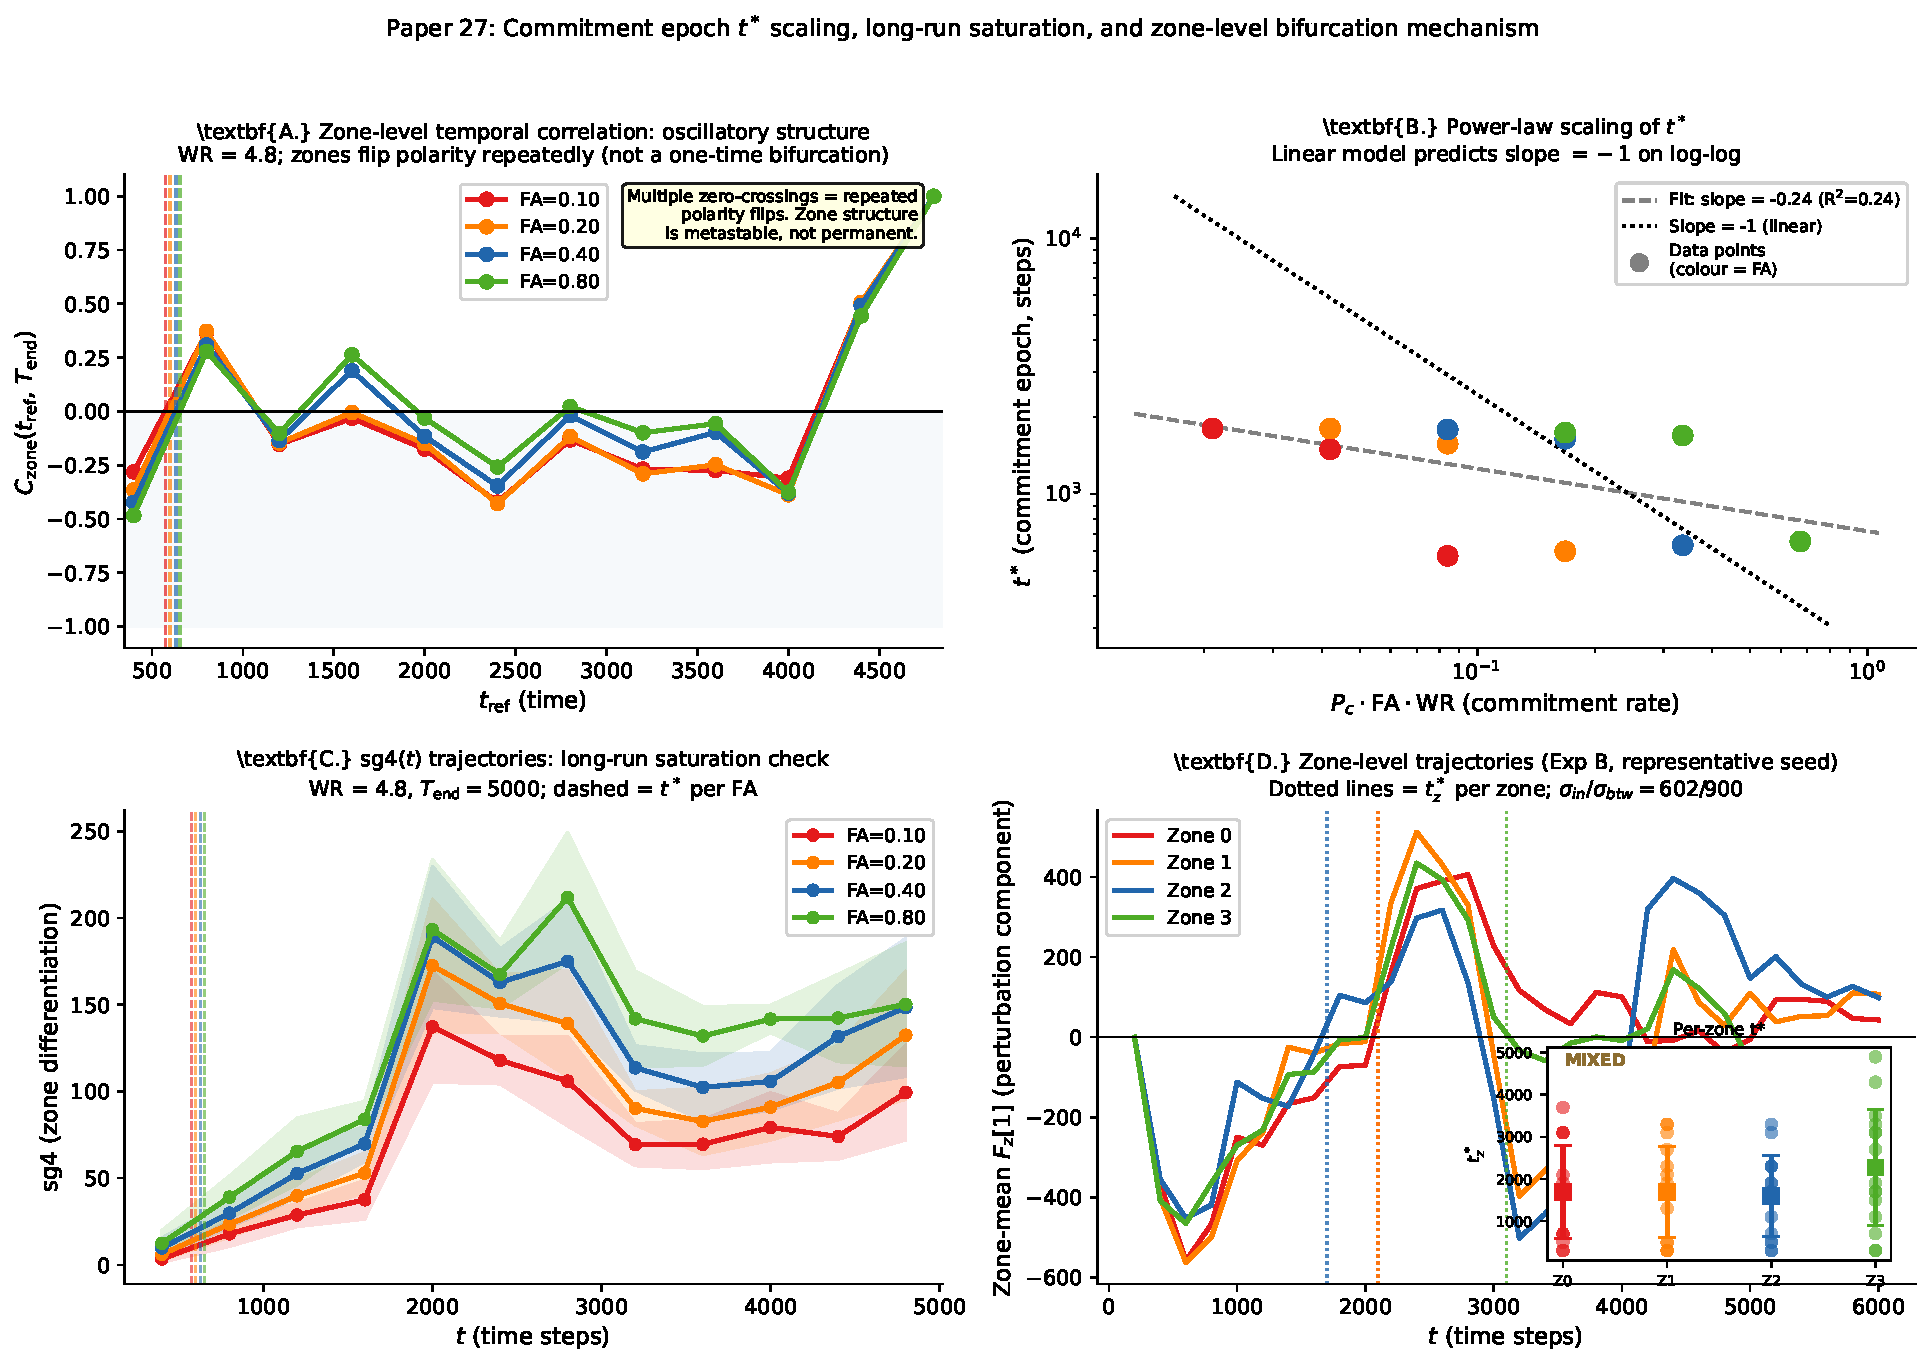
\includegraphics[width=\linewidth]{paper27_figure1.pdf}
\caption{\textbf{Paper 27 summary.}
\textbf{A}: Zone-level temporal correlation $C_{\rm zone}(t_{\rm ref},
  T_{\rm end})$ vs.\ $t_{\rm ref}$ for FA $\in \{0.10,0.20,0.40,0.80\}$,
  WR$=4.8$.  Multiple zero-crossings reveal oscillatory zone polarity.
\textbf{B}: First flip time $t^*$ vs.\ $P_c \cdot \mathrm{FA} \cdot \mathrm{WR}$
  (log-log).  FA-independence visible: points at the same WR cluster vertically
  despite different FA (and hence different x-axis positions).  Slope is set by
  WR variation, not FA variation.
\textbf{C}: sg4$(t)$ for FA $\in \{0.10,0.20,0.40,0.80\}$, WR$=4.8$.
  sg4 continues to grow at $T=5000$; no saturation reached for FA $\geq 0.20$.
\textbf{D}: Zone-mean $F_z[1]$ (perturbation component) vs.\ $t$ for all
  four zones in a representative Exp~B seed.  Polarity flips visible; dotted
  lines mark per-zone $t^*_z$.  Inset: distribution of $t^*_z$ by zone across
  15 seeds, with verdict ``MIXED.''
}
\label{fig:main}
\end{figure}

% ─────────────────────────────────────────────────────────────────────────────
\section{Discussion}
% ─────────────────────────────────────────────────────────────────────────────

\paragraph{Q1 resolved (partially).}
$t^*$ does not scale as $1/(P_c \cdot \mathrm{FA} \cdot \mathrm{WR})$.
The correct scaling is $t^* \approx f(\mathrm{WR})$ with FA contributing
negligibly.  Future work should determine the precise $f(\mathrm{WR})$
functional form over a wider WR range.

\paragraph{Q2 extended.}
sg4 does not saturate within $T=5000$.  The saturation timescale exceeds
5000 steps for standard parameters.  This is consistent with the
amplitude-polarity separation: amplitude (sg4) grows slowly via copy-forward
accumulation, while polarity oscillates on a faster timescale.

\paragraph{Q7 resolved.}
The flip mechanism is a ``noisy pitchfork'': zones flip collectively
(pitchfork-like global instability) but with $\sim 600$ steps of asynchrony
between zones (partial spinodal character).  The dominant variability is
between seeds (random wave history), not between zones within a seed.

\paragraph{Implications for ``critical period.''}
The oscillatory polarity means there is no true ``critical period'' in the
sense of a one-time developmental window.  Instead, the VCML zone structure
is continuously remixing its polarity.  A ``critical period'' would require
suppressing the polarity oscillations -- achievable either by increasing
crystallization (bad: loses amplitude adaptivity) or by adding a symmetry-
breaking mechanism (e.g., asymmetric initial conditions, geographic relay
coupling from V99--V100).

% ─────────────────────────────────────────────────────────────────────────────
\section{Conclusion}
% ─────────────────────────────────────────────────────────────────────────────

Paper~27 resolves three open questions from the theory synthesis, with
surprising answers:
\begin{itemize}
  \item \textbf{Q1}: $t^* \approx f(\mathrm{WR})$, not $1/(P_c\cdot\mathrm{FA}\cdot\mathrm{WR})$.
        Perturbation rate controls timing; consolidation rate controls amplitude.
  \item \textbf{Q2}: sg4 does not saturate within $T=5000$.
        Amplitude and polarity operate on different timescales.
  \item \textbf{Q7}: Mixed pitchfork--spinodal ($\sigma_{\rm in}/\sigma_{\rm btw} = 0.67$).
        Zone flips are collective but asynchronous.
\end{itemize}

The core reframing: VCML zone structure is \emph{metastable}, not
\emph{committed}.  Mandatory turnover drives continuous polarity oscillations
that keep the spatial pattern ergodic.  This is a direct prediction of the
anti-crystallization principle, confirmed at the temporal level.

\end{document}
